\thispagestyle{empty}

\section*{VIGENERE-Tabelle}
\begin{figure}[H]
\centering
\resizebox{1.0\linewidth}{!}{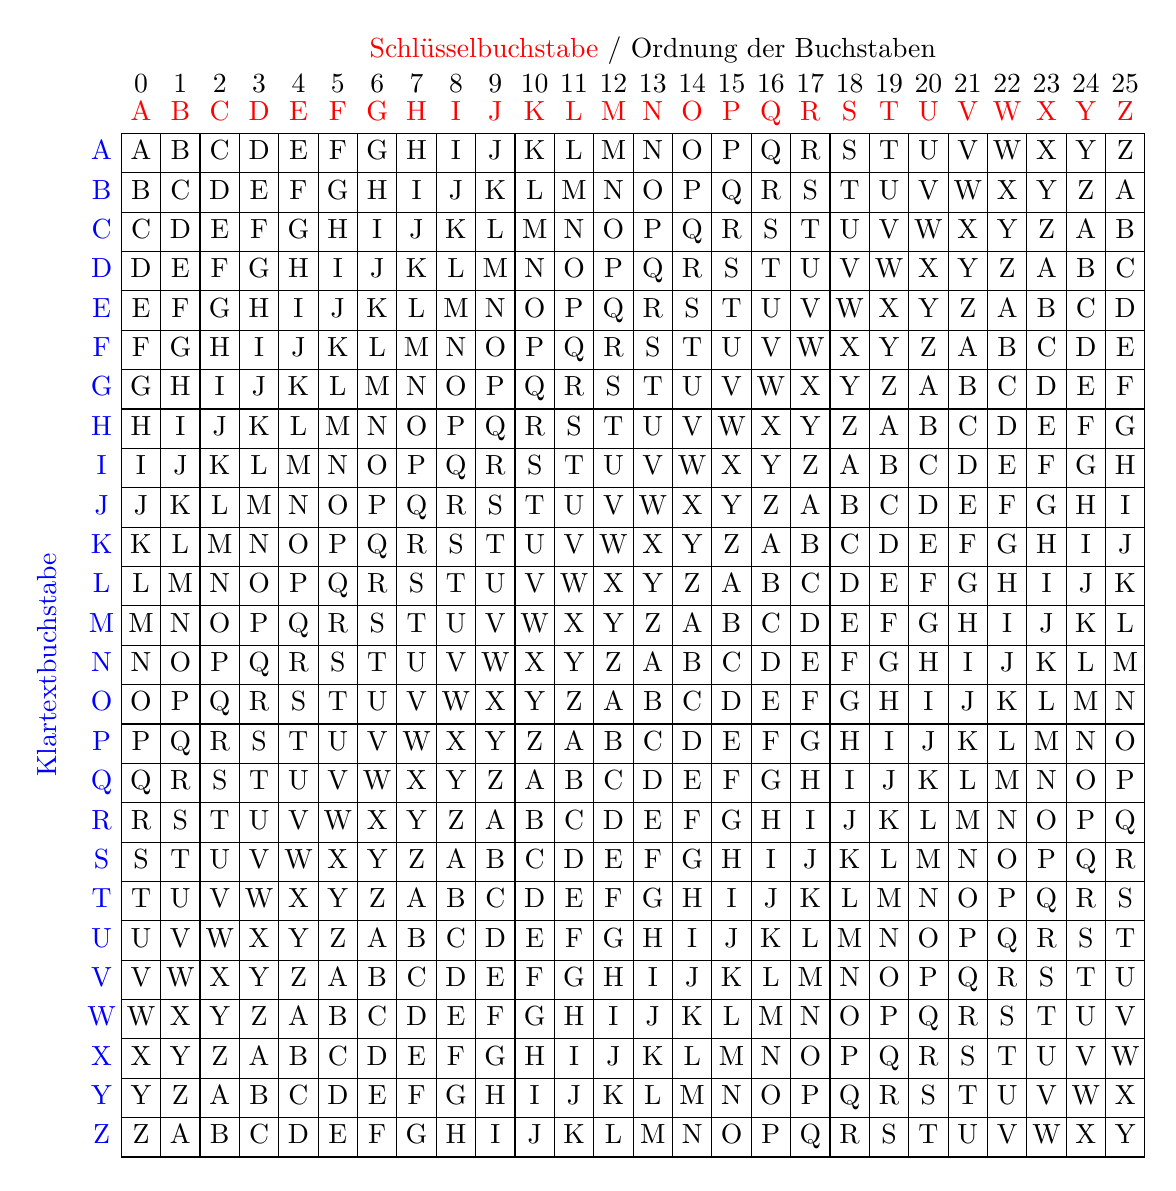
\begin{tikzpicture}
\foreach \i in {0,...,25} {
    \node at (-0.5,-\i*0.5) {\textcolor{Blue}{\strut\symbol{\numexpr`A+\i\relax}}};
    \node at (\i*0.5,0.5) {\textcolor{Red}{\strut\symbol{\numexpr`A+\i\relax}}};
    \node at (\i*0.5,0.85) {\strut\i\relax};
  \foreach \j in {0,...,25} {
    \edef\k{\ifnum\numexpr\i+\j\relax>25
        \the\numexpr\i+\j-26\relax
      \else
        \the\numexpr\i+\j\relax
      \fi}
  \node[draw,minimum size=0.5cm,inner sep=0pt]
    at (\i*0.5,-\j*0.5) {\strut\symbol{\numexpr`A+\k\relax}};
  }
}
% \node[draw,minimum size=0.5cm,inner sep=0pt,fill=Green!20] at (5.0,-2.0) {\textcolor{Green}{O}};
\node at (6.5,1.3) {\textcolor{Red}{Schlüsselbuchstabe} / Ordnung der Buchstaben};
\node[rotate = 90] at (-1.2,-6.5)  {\textcolor{Blue}{Klartextbuchstabe}};
\end{tikzpicture}}
\end{figure}

